\subsection{Controller Subsystem}
\label{sec:controller_subsystem}
% Why the MCU connects to the internet
In order for our system to be as self and power efficient as
possible from an end-user perspective, it was determined that our product
would require an internet connection to offload remote command-and-control
to an Amazon Web Services EC2 instance (hence referred to as "AWS" and detailed in
\autoref{sec:web_subsystem}). To make the process of operating our product 
as hands-off as possible to end-users, the microcontroller will connect to
the user's home WiFi network for access to AWS. Bluetooth, Zigbee, Thread,
and other short-range 2.4 GHz communication protocols were disfavored over
WiFi, as we predict most users will not have a device dedicated to
connecting our product via such protocols. Long range (LoRa) protocols were
deemed unncessary, as the intended placement of our product is outside, 
near or next to the user's home. We do not expect our product to produce
or receive large amounts of data, so the decreased bandwidth of a
WiFi-enabled product being beyond the outdoor walls of a building
is not a significant drawback to our application. A wired connection
(802.3/Ethernet) was deemed too invasive to the end-user. It is expected
that most, if not all, end-users have a wireless access point and internet
access. Thus, connection via the 802.11/WiFi standard was a natural choice
for our use case.

% How the MCU connects to the internet (local network, LAN -> NAT -> WAN,
% TCP stack)
\paragraph{CC3220 Overview}
The Texas Instruments CC3220-series (hence referred to as the "CC3220", the
"MCU", or the "microcontroller") of microcontrollers are WiFi-enabled
chips with an ARM Cortex-M4 central processor and a WiFi network processor,
along with many useful peripherals and power management modules. This
series of processors is delivered alongside a software development kit
(SDK) provided by Texas Instruments to ease the development of
Internet-of-Things (IoT) applications.
\begin{figure}[H]
    \caption{CC3220 embedded software overview (\href{https://www.ti.com/lit/ds/symlink/cc3220s.pdf}{SimpleLink™ Wi-Fi® CC3x20, CC3x3x Network Processor (Rev. M)}, Fig. 1-2)}
    \label{cc3220_sw_overview}
    \centering
    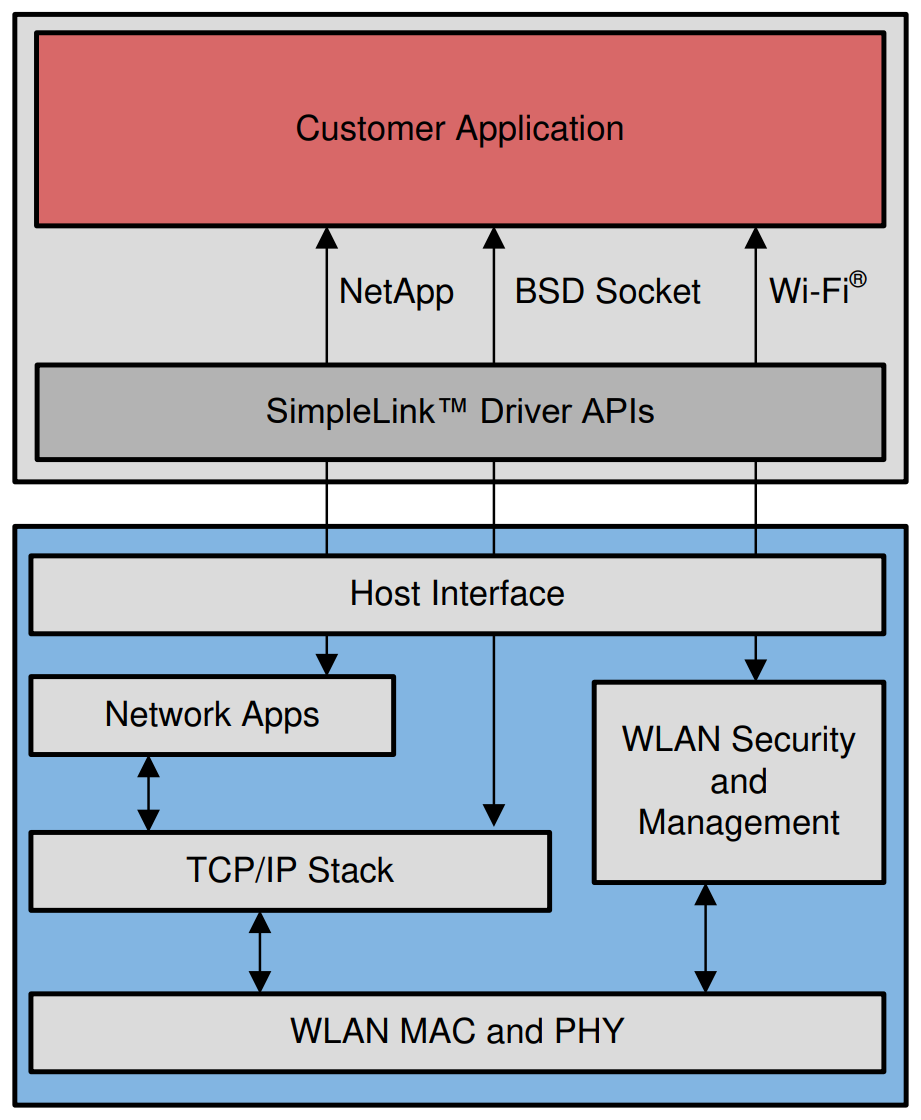
\includegraphics[width=0.75\textwidth]{images/cc3220_sw_overview.png}
\end{figure}
The CC3220's WiFi network processor supports the following
standards/features useful to our development
(see \autoref{cc3220_network_subsystem}):
\begin{itemize}
    \item WiFi standards: 802.11b/g/n
    \item WiFi security: WEP, WPA/WPA2 PSK, WPA2 enterprise, WPA3 personal,
    WPA3 enterprise
    \item WiFi provisioning: SmartConfig, WPS2
    \item IP protocols: IPv4, IPv6
    \item IP addressing: static IP, DHCPv4, DHCPv6
    \item Transport: UDP, TCP, RAW
    \item Host interface: UART, SPI
    \item Built-in transceiver and 2.4 GHz antenna
\end{itemize}
The CC3220's networking subsysem is further detailed in
\autoref{cc3220_network_subsystem}.
\begin{figure}[H]
    \caption{CC3220 networking subsystem (\href{https://www.ti.com/lit/ug/swru455m/swru455m.pdf}{CC3220 SimpleLink™ Wi-Fi® and Internet of Things Technical Reference Manual})}
    \label{cc3220_network_subsystem}
    \centering
    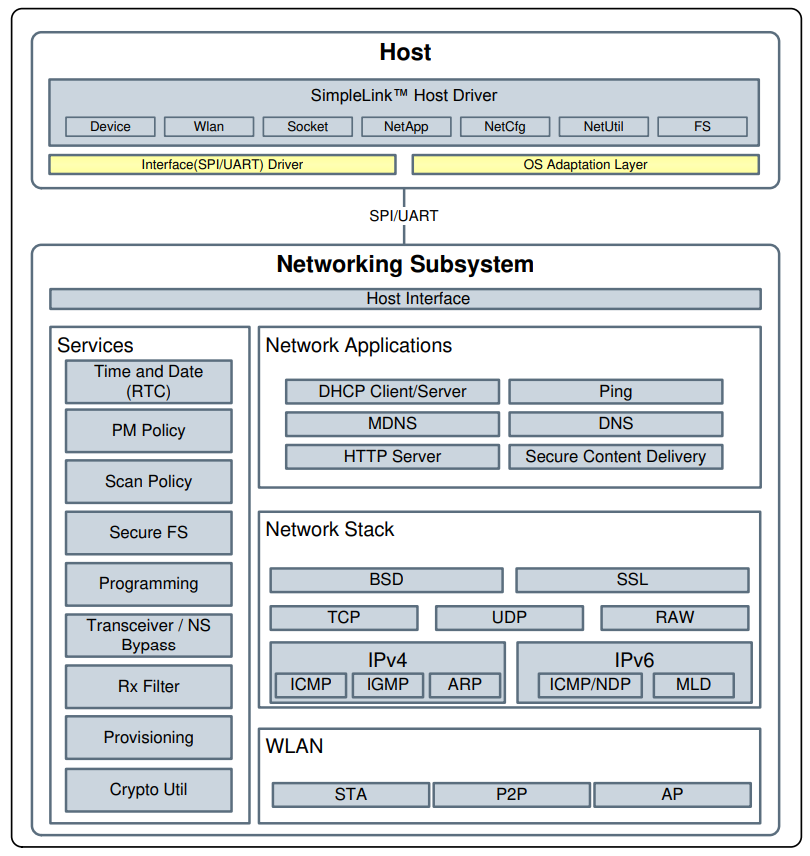
\includegraphics[width=0.75\textwidth]{images/cc3220_network_subsystem.png}
\end{figure}
\paragraph{Connection}
During development of our product, our microcontroller will be hardcoded
for the selected WLAN it will access. In the future, there are multiple
options our team will be able to explore to allow our product to connect to
a wide variety of networks. 

% option a) web interface for user to long in to WLAN
\paragraph{Web Interface Option}
The first option would allow unanimous adaptation of
our product for home users. This option consists of performing first-time
setup through a WiFi Direct connection to the MCU and allowing the user
to login through a web portal to finish setup of their device. The portal
would allow a user to connect to their WLAN of choice, and would
also allow the user to login to the MCU locally to view telemetry and 
settings. The user would also be able to configure the MCU for static
IP addressing or DHCP IP addressing.

% option b) WPS button
\paragraph{WPS Option}
The second option would be to implement a momentary switch which is
programmed to connect to the MCU's WiFi Protected Setup (WPS) feature.
This would still allow the user to connect to their network of
choice---however, the user's wireless access point (WAP) would need to
support WPS. Furthermore, DHCP IP addressing would be forced, and there
would be no web portal for the user to access for viewing telemetry and
settings. This option would greatly ease development, though, and would
let the MCU and web teams focus on developing and refining their
respective subsystems.

% TCP sockets
\paragraph{Communication Method}
The MCU will communicate with AWS through TCP sockets. After connection to
the user's home network, the MCU will check if there is an internet
connection. Once an internet connection has been established, the MCU will
open a socket and connect to the AWS instance via its URL (using the
default DNS nameserver provided to network clients). The software control
flow of TCP sockets as our product will implement them is detailed in
\autoref{tcp_socket_flow}.
\begin{figure}[H]
    \caption{TCP socket control flow (\href{https://www.ti.com/lit/ds/symlink/cc3220s.pdf}{SimpleLink™ Wi-Fi® CC3x20, CC3x3x Network Processor (Rev. M)}, Fig. 6-1)}
    \label{tcp_socket_flow}
    \centering
    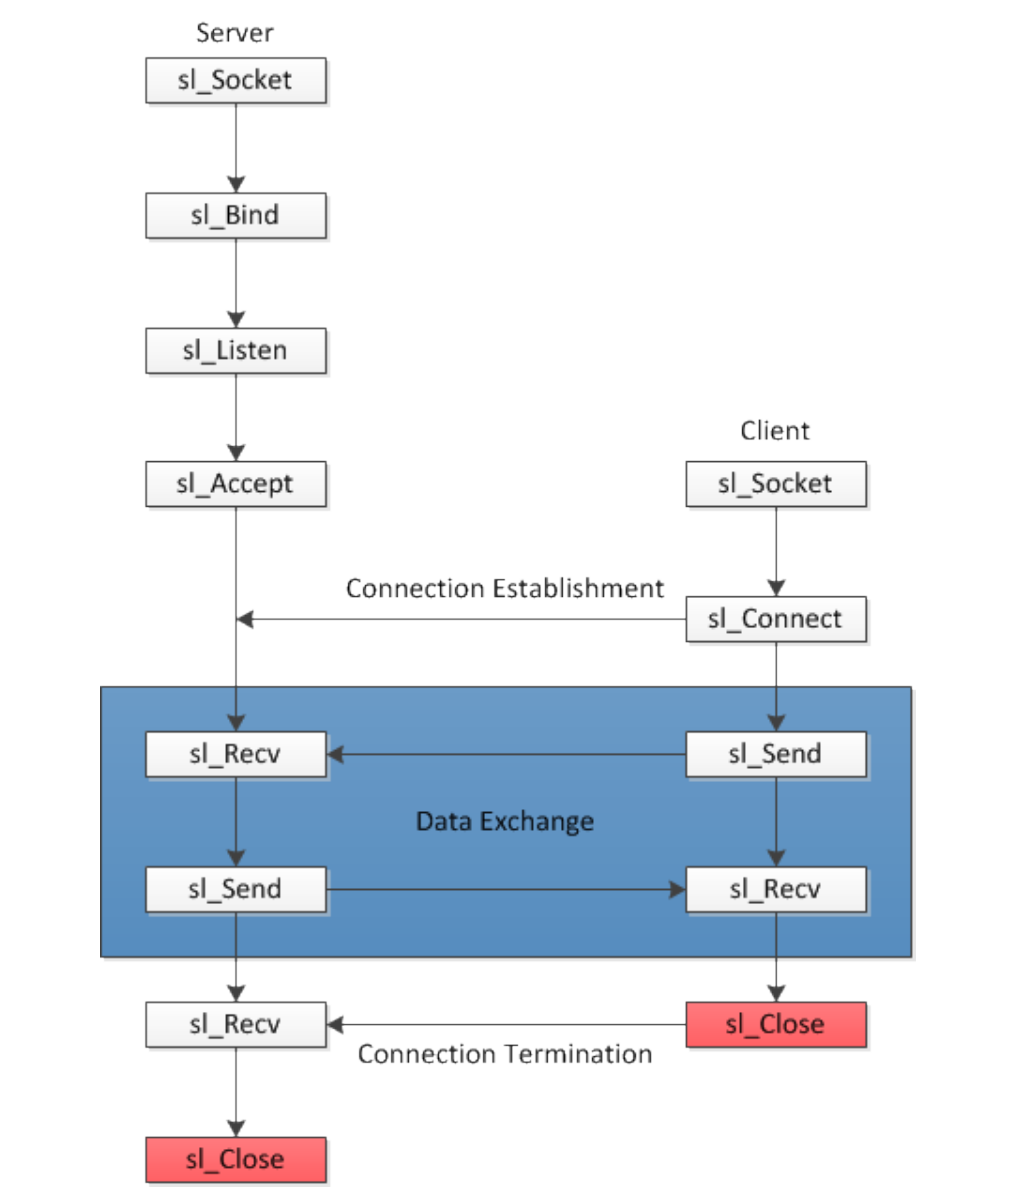
\includegraphics[width=\textwidth]{images/tcp_socket_flow.png}
\end{figure}

% Parameters for connection and how often it tries
\paragraph{Connection Parameters}
Once the MCU has established a connection to the internet and the AWS
instance, it attempts to send current system settings and telemetry, as
well as sensor readings to AWS. The microcontroller does this at least
once every 15 minutes. Sending and receiving may occur more often if
commanded to by AWS. Because TCP is being used to connect AWS and the
microcontroller, any manual retries on a failed send or receive most
likely will be futile. Therefore, any sort of link error handling will
be performed by the link and not the microcontroller program.

% Any over-the-air updates?
\paragraph{Over-the-Air Updates}
At this time, our team does not intend to provide a method for over-the-air
updates (OTA), however, this is a provision that may be developed in the
future.

% MCU receives commands, decodes commands
\paragraph{Commands from AWS}
The MCU will receive commands and data from AWS in the following form:
\begin{center}
    \texttt{t x c y}
\end{center}
where \texttt{t} (character) marks the beginning of the command string,
\texttt{x} (unsigned integer) indicates how many seconds to wait before
executing command \texttt{c} (character) with parameter \texttt{y}
(ambiguous). The following characters occupy the spot of \texttt{c}, and
translate to the following commands:
\begin{center}
    \texttt{w y}: water, \texttt{y} is boolean \\
    \texttt{a y}: solar $\theta$, \texttt{y} is double \\
    \texttt{b y}: solar $\phi$, \texttt{y} is double \\
    \texttt{l y}: low power, \texttt{y} is unsigned int for flags \\
    \texttt{s y}: send data, \texttt{y} is unsigned int for flags
\end{center}
For example, if AWS instructs the MCU to turn on the water source in 3
minutes, it would send the command \texttt{t 180 w 1}. If AWS would like
the MCU to change the $\theta$ of the solar panels to 45$\degree$
immediately, it would send \texttt{t 0 a 45.0}. It is important to note
that the values of \texttt{x} and \texttt{y} are not strings (e.g.
45$\degree$ will not be sent as \texttt{"45.0"}), but the actual encoding
of 45$\degree$ as a double-precision float. This is to maintain a
consistent command string size amongst all transmissions.
\begin{figure}[H]
    \caption{Bitwise representation of command}
    \label{command_bitwise}
    \centering
    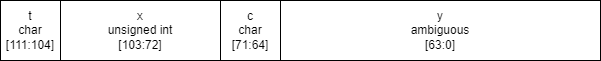
\includegraphics[width=\textwidth]{images/command_encoding.png}
\end{figure}

% Will program in C++. Any libraries, multithreading?
% Singleton Pattern Thread for scheduling tasks
\paragraph{C++ Structure}
It should be expected that all headers from the C++ standard library (as
defined in C++20) will be used, along with the following nonstandard
libraries: Texas Instruments SimpleLink™ CC32xx SDK. Additionally, it is
expected that the MCU program will schedule tasks using a Singleton Pattern
thread to ensure thread safety when accessing variables.

% Classes and class diagram
\paragraph{Classes}
There will be a few classes defined in the MCU's programming, detailed
in \autoref{classes_uml}. Classes will be laid out in the header file
according to the definitions given in the UML diagram.
\begin{figure}[H]
    \caption{UML diagram of the classes used}
    \label{classes_uml}
    \centering
    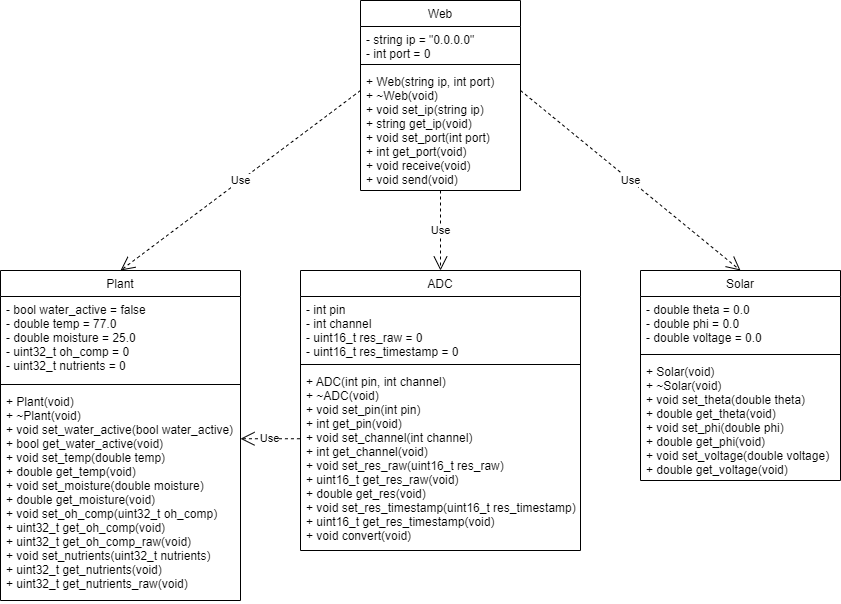
\includegraphics[width=\textwidth]{images/classes_uml.png}
\end{figure}

% Web class
\paragraph{Web Class}

% Plant class
\paragraph{Plant Class}

% Solar class
\paragraph{Solar Class}

% ADC class
\paragraph{ADC Class}

% Send to AWS, format and types of commands
% Send straight data from the struct
\paragraph{Data to AWS}
Unlike commands received from AWS, the MCU will simply send data directly
from its classes to AWS. This is done to minimize the overhead of sending
extraneous symbols and preserve power stored in the battery, as receiving
uses far less power than transmitting in the MCU subsystem. Further
optimization can be performed in the future to further reduce overhead
(e.g. reducing \texttt{water\_active} to occupy 1 bit and using the rest of
the symbol to encode other data).
\begin{figure}[H]
    \caption{Bitwise representation of data sent to AWS}
    \label{toweb_encoding}
    \centering
    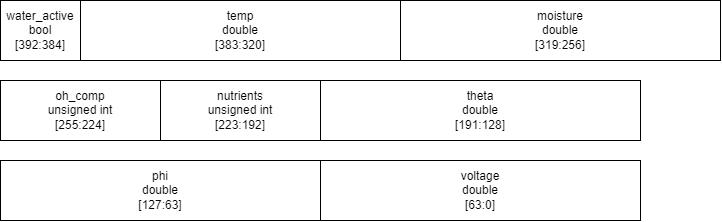
\includegraphics[width=\textwidth]{images/toweb_encoding.png}
\end{figure}

% Global vars
\paragraph{Global Variables}
No global variables plan to be implemented at this time. Macros may be
defined for configuration of the ADC and any other dependent modules.

% Interrupts and ISRs
\paragraph{Interrupts and ISRs}
If the charge controller indicates that the battery has fallen below a
certain voltage (named "low voltage"), the MCU will raise an interrupt and
execute \texttt{isr\_low\_power()}. This ISR performs housekeeping before
putting the MCU into a low power state, limiting use of its functions.

% Interrupts and ISRs (cont.)
If the charge controller indicates that the battery has fallen below a
certain voltage (named "critical voltage"), the MCU will raise an interrupt
and execute \texttt{isr\_critical\_power()}. This ISR performs further 
housekeeping before putting the MCU into an extreme low power state,
limiting all but the features necessary to maintain a connection with AWS.

% Interrupts and ISRs (cont.)
If the MCU, AWS, or any other devices transmit indication of a dangerous
state or if the MCU, AWS, or any other devices transmit indication of a
shut down, the MCU will raise an interrupt and execute
\texttt{isr\_shut\_down()}. This ISR immediately shuts down all able
subsystems, and puts all other subsystems in a fail safe state. This ISR
fails safe the entire system.

% Interrupts and ISRs (cont.)
If the MCU receives indication of a start up (via a momentary switch), the
MCU will raise an interrupt and execute \texttt{isr\_start\_up()}. This ISR
starts up all relevant subsystems and begins the MCU's programming. All
classes will be initialized to default values. This ISR starts up the
entire system.

% Interrupts and ISRs (cont.)
If the MCU determines it must reset the system to a default state, the
MCU will raise an interrupt and execute \texttt{isr\_default\_state()}.
This ISR returns all relevant subsystems to their default state,
as if the MCU had just executed \texttt{isr\_start\_up()}. All classes will
be initialized to default values. This ISR resets the entire system.

% File organization (main, header files, other source files, etc.)
\paragraph{File Organization}
Classes, macros, functions, and variables will be defined/prototyped to the
extent required in a header file to be named \texttt{garden.h}. These
classes, functions, and variables will be further defined in a seperate
source file named \texttt{garden.cpp} as needed. The \texttt{main()}
function and the remaining classes, macros, functions, and variables,
required will be located in \texttt{main.cpp}.

% How the MCU gets data from sensors (ADC)
\paragraph{Analog-to-digital Conversion}
The CC3220 contains a 12-bit general purpose analog-to-digital converter
(ADC) with 4 externally-accessible channels and a sampling periodicity of
16 $\upmu$s per channel (62.5 ksps per channel). The architecture of the
CC3220's ADC is shown in \autoref{cc3220_adc_arch}.
\begin{figure}[H]
    \caption{CC3220 ADC module architecture (\href{https://www.ti.com/lit/ug/swru465/swru465.pdf}{CC3220 SimpleLink™ Wi-Fi® and Internet of Things Technical Reference Manual}, Fig. 13-1)}
    \label{cc3220_adc_arch}
    \centering
    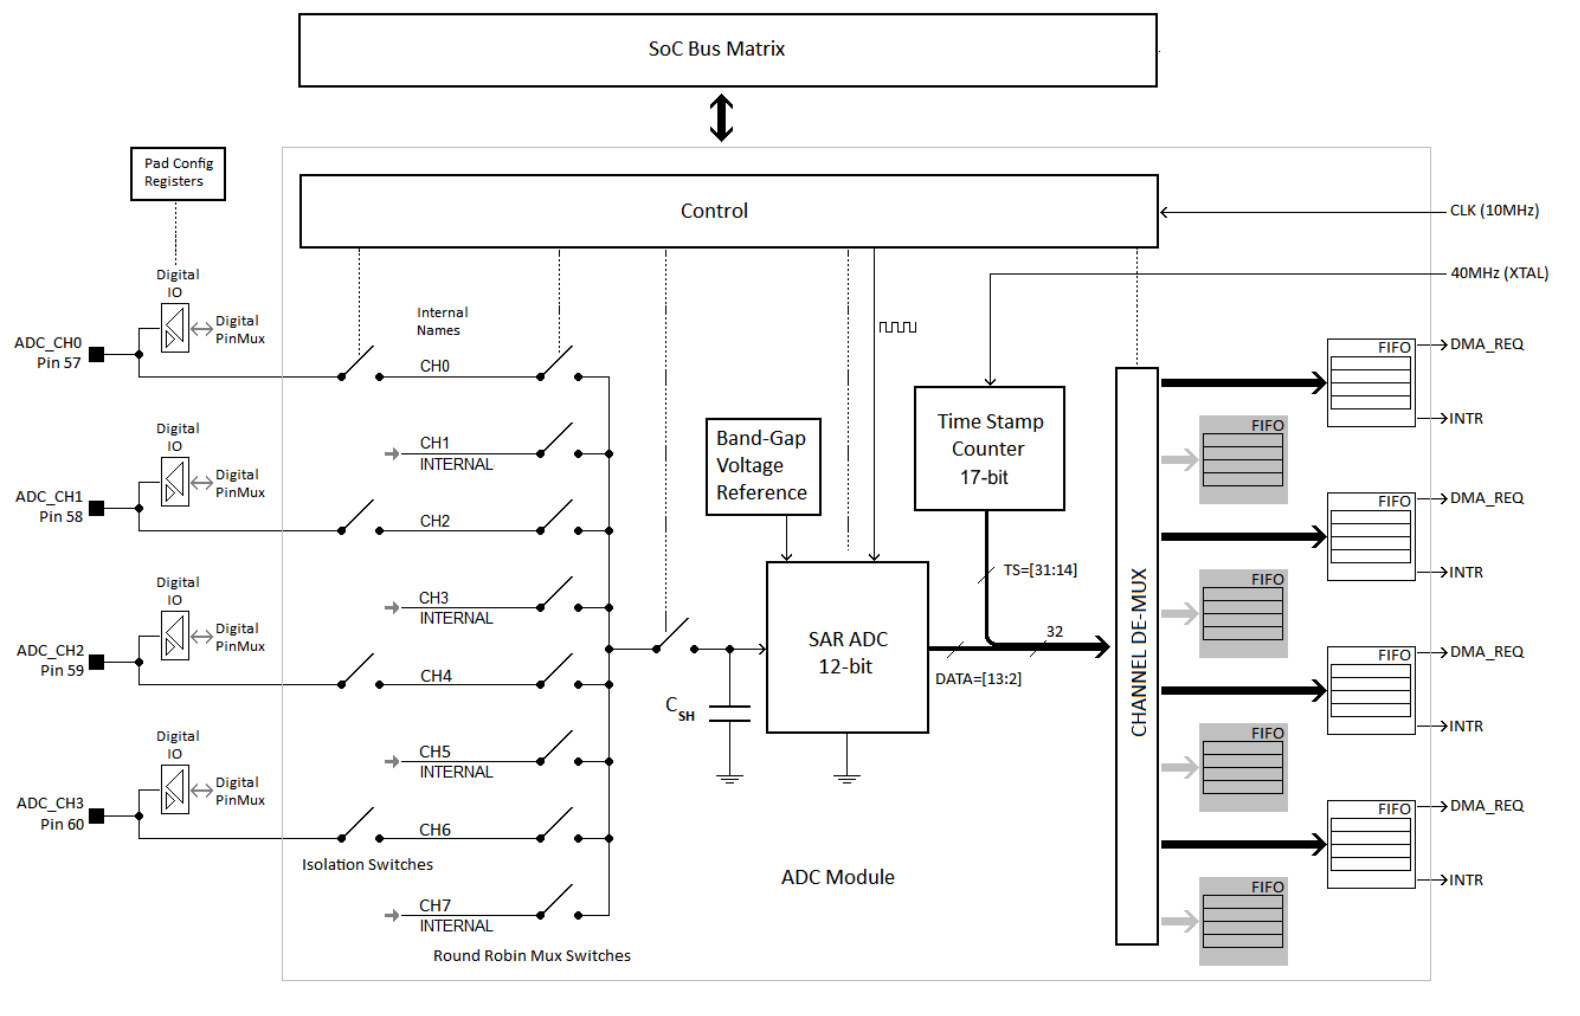
\includegraphics[width=\textwidth]{images/cc3220_adc_arch.png}
\end{figure}

% How the MCU gets data from sensors (ADC, cont.)
It is expected that the spectrometer circuit will provide a current
between 20 $\upmu$V and 80 mV. The 12-bit ADC provides for an input range of
between 0 and 1.8 V. Therefore, the resolution of the ADC is calculated
below:
\begin{equation}
    \label{eq:adc_res}
    \frac{(1.8 - 0)\,\mathrm{V}}{2^{12}\,\mathrm{steps}} =
    0.4395\,\mathrm{mV}/\mathrm{step}
\end{equation}
Thus, given our ADC resolution and the expected range of our spectrometer,
the number of discrete steps of range is given below:
\begin{equation}
    \label{eq:adc_steps}
    \frac{(80 - 0.02)\,\mathrm{mV}}{0.4395\,\mathrm{mV}/\mathrm{step}} =
    \lfloor181.98\rfloor = 181
\end{equation}
These steps will be used to measure OH composition and nutrients in the
soil, and functions from the class \texttt{ADC} will be used to perform
analog-to-digital conversion to update values in the class \texttt{Plant}.

In the future, a more precise ADC module could be explored to give the
CC3220 more resolution when performing spectroscopy.

% How MCU sends data to servos
\paragraph{Communication with Servos}
The MCU will directly control GPIO and bit-bang values to the servo motors
controlling the orientation of the solar panels when using functions from
the class \texttt{Solar}. This method of control may be refined further in
the future.

% What sort of telemetry we'll have
\paragraph{Telemetry}
No data that would be exclusively considered telemetry will be transmitted 
between AWS and the MCU (e.g. processor temperature). Instead, all
"telemetry" values will be handled with interrupts and ISRs/functions
on-chip, while current settings and sensor readings will be transmitted
back to AWS.

% What kind of development model?
\paragraph{Development Model}
An Agile development model will be used. Code reviews will be performed on
an as-needed basis by a convening of members of the MCU subsystem and the
web subsystem teams.
\begin{figure}[H]
    \caption{UML diagram of the subsystem's development methodology}
    \label{mcu_agile_uml}
    \centering
    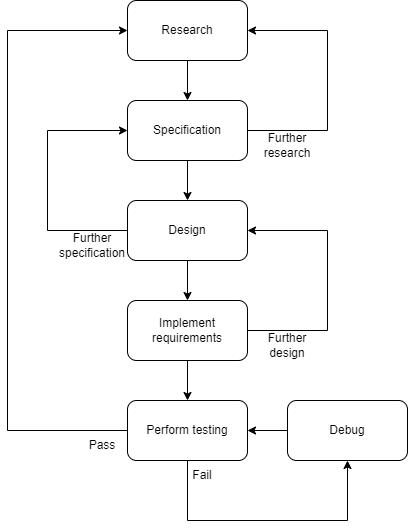
\includegraphics[width=0.75\textwidth]{images/mcu_agile_uml.png}
\end{figure}

% IDE and Git
\paragraph{IDE and Git}
Texas Instruments Code Composer Studio v12 will be used to program,
compile (via TI ARM compiler v20), and debug the C++-based project. GitHub
will be used as a repository for the project, using Git for version
control.
